% RQ-organized revision based on the user manuscript of 23 September 2026.
% No new scientific experiments. Exact source and editorial decisions are
% provenance: ../migration/COMPLETION_SOURCE_MAP_20261003.json (author records).
\documentclass{article}
\usepackage{iclr2027_conference,times}
\usepackage[T1]{fontenc}
\usepackage[utf8]{inputenc}
\usepackage{amsmath,amssymb,mathtools,booktabs,array,multirow}
\usepackage{graphicx,xcolor,algorithm,algpseudocode}
\usepackage{microtype}
\usepackage{hyperref,url}
\definecolor{LinkBlue}{HTML}{1955A5}
\hypersetup{colorlinks=true,citecolor=LinkBlue,linkcolor=LinkBlue,
 urlcolor=LinkBlue,pdfborder={0 0 0},
 pdftitle={Acoustic-to-KV Regression for Bioacoustic Recognition in Speech Language Models},
 pdfauthor={Anonymous authors}}
\newcommand{\method}{AKR}
\newcommand{\R}{\mathbb R}
\newcommand{\Sset}{\mathcal S}
\newcommand{\Qset}{\mathcal Q}
\newcommand{\Aset}{\mathcal A}
\newcommand{\norm}[1]{\left\lVert#1\right\rVert}
\newcommand{\pp}{\,\mathrm{pp}}
\newcolumntype{L}[1]{>{\raggedright\arraybackslash}p{#1}}
\title{Acoustic-to-KV Regression for\\
Bioacoustic Recognition in Speech Language Models}
\author{Anonymous authors}
%\iclrfinalcopy
\begin{document}
\maketitle
\lhead{Under review as a conference paper at ICLR 2027}

\begin{abstract}
Animal-sound recognition requires distinguishing call types, callers, and species from acoustic evidence. Speech language models can encode these distinctions without reliably selecting the corresponding text labels. On marmoset queries, a ridge classifier fitted to two labelled clips from each of six call types reaches 58.67\% using frozen Qwen2.5-Omni features; audio in-context learning receives the same clips but reaches 17.33\%, predicting one class throughout. This exposes a gap between usable acoustic representations and native label prediction. We introduce \emph{Acoustic-to-KV Regression} (\method) to help the frozen model use its acoustic features when selecting a label. Correct-answer gradients from labelled support recordings provide internal correction targets. A low-rank ridge map predicts their coordinates from acoustic features and adds the reconstructed increments to audio-token K/V states before generation, without query labels, query backpropagation, or backbone updates. In five recording-group evaluations of 1-kHz marmoset recognition with error-enriched support, \method\ raises mean accuracy from 12.35\% to 32.47\% and macro-F1 from 5.92\% to 24.54\%, outperforming native generation and a fixed correction in every evaluation. Separate held-out-support analyses reduce gradient-prediction error by 31.87\% on Full input and 23.59\% at 1\,kHz relative to the fixed mean. Together, these results connect accessible acoustic information to learnable state corrections that improve native recognition in the studied settings.
\end{abstract}

\section{Introduction}
Animal-sound recognition is more specific than deciding whether a recording contains a monkey, a dog, or a whale. Within the common marmoset species, a Phee is a sustained tonal call, a Trill contains repeated frequency modulation, and a Twitter comprises separated upward sweeps. Their distinction involves duration and frequency--time structure, not simply pitch \citep{dimattina2006virtual,agamaite2015quantitative}. Identifying which dog produced a bark is a different task: its label denotes a caller rather than a call type. These tasks help organize vocal repertoires and identify sound sources in bioacoustic analysis \citep{lamothe2025marmaudio,hagiwara2022beans}. They also provide a concrete test of whether a generalist speech language model can connect detailed acoustic evidence to the appropriate text label.

Consider learning MarmAudio's six call types from two labelled recordings per type: twelve audio--label pairs from the same species. A ridge classifier fitted to frozen Qwen2.5-Omni features reaches 58.67\% on recording-disjoint queries. Native audio in-context learning (ICL) receives exactly the same examples but reaches 17.33\%, predicting one class throughout (Figure~\ref{fig:motivation}b). These examples support useful acoustic classification, yet the model's own answer process uses them poorly. Matching the recordings and labels makes this a comparison of how supervision is used, rather than how much annotation each route receives.

\begin{figure}[t]
\centering
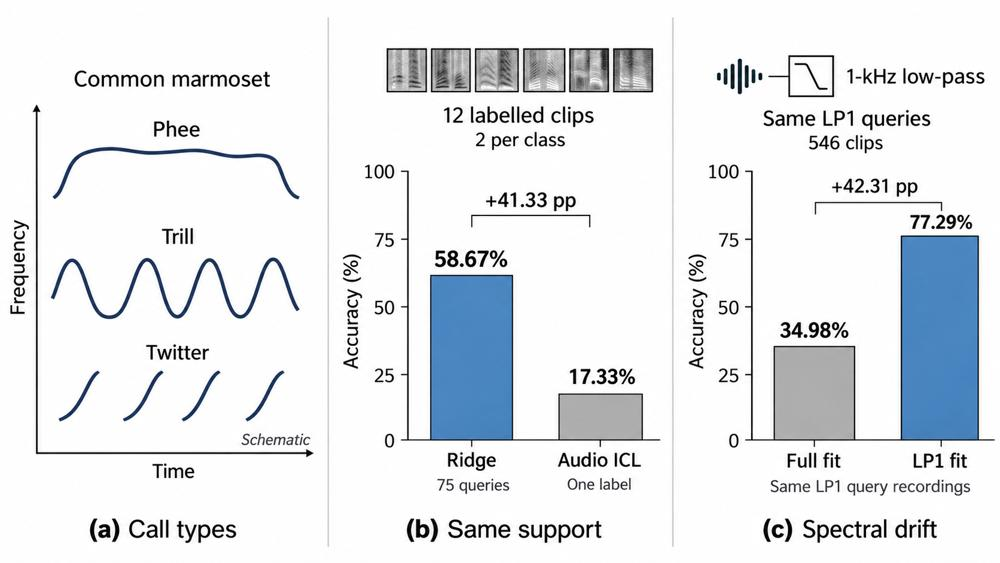
\includegraphics[width=\linewidth]{figures/intro.jpg}
\caption{\textbf{Two observations motivate internal correction.} (a) Schematic call structures within one species. (b) An explicit readout outperforms native audio ICL given identical support. (c) The same low-pass queries remain classifiable, but a Full-trained readout transfers poorly. Protocols are in Appendix~\ref{app:diagnosis}.}
\label{fig:motivation}
\end{figure}

A separate recording-grouped probe experiment tests what happens when the available spectrum changes. We low-pass filter MarmAudio recordings at 1\,kHz while retaining their class labels. On identical filtered queries, a classifier fitted to 1-kHz training features reaches 77.29\%, whereas a Full-trained classifier transferred unchanged reaches 34.98\% (Figure~\ref{fig:motivation}c). We call this readout-transfer deficit \emph{spectral decision drift}: the representation remains useful for classification, but the earlier readout no longer uses it as effectively. Related discrepancies occur for individual dogs and marine-mammal species. Appendix~\ref{app:diagnosis} defines both diagnostics and reports their separate protocols; this spectral probe study is not the twelve-example ICL experiment.

Together, these observations motivate a concrete question: \emph{can a new recording's acoustic features predict an internal correction that helps the frozen model select the right label?} A labelled support recording supplies not only its category, but also a correct-answer loss whose gradient describes how internal states should move locally to favour that answer. We use this signal to learn a correction predictor, rather than replace the model's output classifier.

Our method, \emph{Acoustic-to-KV Regression} (\method), compresses support-derived correction targets into a low-rank basis and fits a ridge map from frozen acoustic features to their coordinates. At inference, it predicts a recording-specific increment and lets the original model generate the label. The experiments follow this construction: we first evaluate end-to-end recognition, then test the value of input conditioning, and finally measure whether acoustic features predict held-out correction targets. This separates a useful representation, a learnable correction, and an improvement in the model's actual answer.

Our contributions are as follows:
\begin{itemize}
\item \textbf{We identify and quantify spectral decision drift.} Condition-fitted and transferred readouts on identical filtered recordings distinguish retained acoustic discrimination from the applicability of an existing classifier. Matched-support ICL comparisons provide complementary evidence of underused acoustic supervision.
\item \textbf{We propose Acoustic-to-KV Regression.} Low-rank coordinates of negative answer-loss gradients supervise a ridge map from frozen acoustic features to additive K/V increments. The backbone remains fixed, and new recordings require neither labels nor backward passes.
\item \textbf{We connect recognition gains to controlled and predictive evidence.} \method\ improves mean 1-kHz marmoset accuracy by 20.12 percentage points across five recording-group evaluations. Dogs controls test input conditioning at matched relative norms, and held-out gradient prediction supports the acoustic-to-correction map.
\end{itemize}

\section{Related Work}
\paragraph{Spectral robustness and decision mismatch in speech language models.}
Speech language models must convert acoustic representations into language-side decisions. Analyses of the speech--text modality gap show that representation alignment alone does not ensure stable answer selection \citep{hsu2026modality}. Audio-specialist-head steering increases the influence of acoustic evidence through audio--silence activation contrasts \citep{glazer2026heads}; KV-cache steering controls frozen language models through inference-state interventions \citep{belitsky2025kv}. Beyond the Baseband instead encodes higher-frequency bands excluded by low-rate inputs \citep{sarkar2026baseband}. We examine changes within the model-observable band: whether class information remains usable after filtering when an existing readout fails to transfer. This readout-level diagnosis motivates, but is distinct from, evaluating corrections through the native decoder.

\paragraph{Few-shot learning and support utilization.}
Audio Flamingo demonstrates audio ICL and retrieval-based adaptation \citep{kong2024audioflamingo}. MetaSICL strengthens auditory models' contextual adaptation through post-training on high-resource speech, while FSA-GRPO rewards effective use of demonstrations \citep{zheng2026metasicl,zheng2026fsagrpo}. These approaches treat the ability to use examples as a capability that can itself be learned. We compare explicit fitting and native ICL under identical acoustic supervision. Rather than post-train the speech model to consume demonstrations, \method\ fits a predictor of support-derived internal corrections. Predicting backward signals is related to synthetic-gradient methods \citep{jaderberg2017synthetic}, but our predicted quantities modify a frozen model's inference states rather than decouple weight optimization.

\paragraph{Bioacoustic recognition and language interfaces.}
BEANS standardizes animal-sound classification and detection, MarmAudio supplies within-species vocal categories, and AVES learns transferable representations from unlabelled recordings \citep{hagiwara2022beans,lamothe2025marmaudio,hagiwara2022aves}. NatureLM-audio connects bioacoustic training to language interaction and introduces BEANS-Zero for unseen taxa and tasks \citep{robinson2025naturelm}. Our focus is an existing generalist speech language model rather than a new bioacoustic foundation model. Call-type, caller, and species labels test whether acoustic distinctions can be associated with appropriate text answers. Probes reveal accessible information, not necessarily information already used by native generation; their supervision and interpretation therefore require explicit controls \citep{hewitt2019probes}.

\section{Acoustic-to-KV Regression}
\label{sec:method}
\method\ learns how a recording should change a frozen model's internal states. Let $\theta$ denote the model parameters, $p$ the task prompt, and $\Sset=\{(x_i,y_i)\}_{i=1}^{n}$ the labelled support recordings. The pooled audio-token representation is $h_i=h_\theta(x_i,p)\in\R^d$. Support fitting extracts corrective targets and learns a map from $h_i$ to those targets. For a new recording, the fitted map predicts an increment before the original decoder generates its label (Figure~\ref{fig:method}).

\begin{figure}[t]
\centering
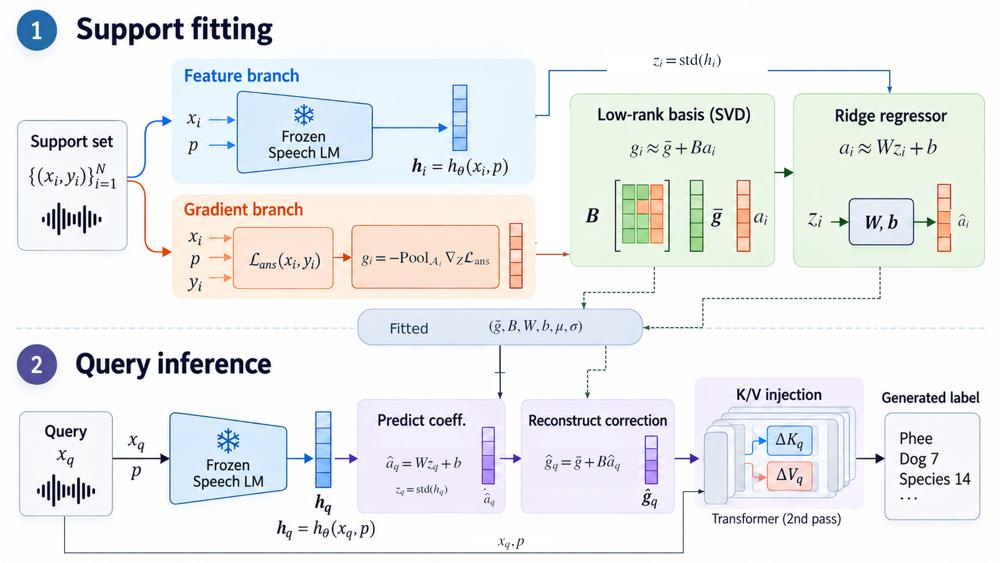
\includegraphics[width=\linewidth]{figures/pipeline.jpg}
\caption{\textbf{Support-fitted correction, native query output.} A feature branch supplies regressor inputs; a labelled answer-loss branch supplies corrective K/V targets. A compact fitted map predicts query-specific increments for the second forward pass. The speech model remains frozen.}
\label{fig:method}
\end{figure}

\subsection{Extract corrective targets from support answers}
Let $Z^s_{i,\ell,t}$ be the output of a selected K/V projection at layer $\ell$, audio position $t$, and type $s\in\{K,V\}$. Interventions act before head reshaping and, for keys, rotary position encoding. Write $\Aset_i$ for the expanded audio-token positions. For the tokenized class name $y_i=(y_{i,1},\ldots,y_{i,m_i})$, the support answer loss is
\begin{equation}
\mathcal L_{\rm ans}(x_i,y_i;p)
=-\frac{1}{m_i}\sum_{j=1}^{m_i}
\log p_\theta(y_{i,j}\mid x_i,p,y_{i,<j}).
\label{eq:answerloss}
\end{equation}
Only answer tokens contribute to this loss. We differentiate it with respect to the projection states, take the negative gradient, pool over audio positions, and concatenate the selected blocks:
\begin{equation}
g^s_{i,\ell}=-\frac{1}{|\Aset_i|}\sum_{t\in\Aset_i}
\frac{\partial\mathcal L_{\rm ans}}{\partial Z^s_{i,\ell,t}},
\qquad
 g_i=\operatorname{concat}_{\ell,s}g^s_{i,\ell}\in\R^P.
\label{eq:gradient}
\end{equation}
The gradient supplies a locally corrective direction, not another category label. Pooling gives a fixed-width target across recordings with different audio-token counts. No backbone optimizer step is taken. The feature branch extracts $h_i$ from the recording and prompt without conditioning its input on the correct answer; the separate labelled branch defines the supervision for correction learning.

\subsection{Fit low-rank acoustic regression}
Stack the correction targets as rows of $G\in\R^{n\times P}$ and let $\bar g=n^{-1}\sum_i g_i$. A thin singular value decomposition of the centred targets defines an orthonormal correction basis:
\begin{equation}
G-\mathbf1\bar g^\top=U\Sigma V^\top,
\qquad B=V_{:,1:r},
\qquad a_i=B^\top(g_i-\bar g),
\label{eq:svd}
\end{equation}
where $B\in\R^{P\times r}$ and $r\leq n-1$. The basis describes variation among support corrections; it does not project the model's original K/V states. We standardize features using support-only means and scales to obtain $z_i$, then fit an affine ridge map \citep{hoerl1970ridge}:
\begin{equation}
(W^*,b^*)=\arg\min_{W,b}
\left[\sum_{i=1}^{n}\norm{Wz_i+b-a_i}_2^2
+\lambda\norm{W}_F^2\right].
\label{eq:regression}
\end{equation}
Thus the two objectives have different roles. Answer cross-entropy produces the correction targets, while squared-error regression learns to predict their coordinates. Although recognition labels are discrete, $a_i\in\R^r$ contains signed real-valued update coefficients. The fitted objects are the feature normalizer, $\bar g$, $B$, $W^*$, and $b^*$; all parameters of the speech model remain unchanged.

\subsection{Predict and apply a query-specific increment}
A first forward pass extracts the unlabelled query feature. After support-based standardization, its predicted correction is
\begin{equation}
\boxed{\widehat g_q=\bar g+B(W^*z_q+b^*).}
\label{eq:prediction}
\end{equation}
We unflatten this vector into K/V blocks. During a second forward pass of the same recording and prompt, a raw step $\eta$ applies the pooled increment at audio positions:
\begin{equation}
Z^{s\prime}_{q,\ell,t}
=Z^s_{q,\ell,t}
+\eta\,\mathbf1[t\in\Aset_q]\,\widehat g^s_{q,\ell}.
\label{eq:update}
\end{equation}
The original decoder then generates the label. The increment varies between recordings, while its pooled vector is shared across the audio positions of a block. Query labels and query-time backward passes are absent from this procedure. This is supervised support fitting followed by inference-state adaptation, not an entirely training-free method.

Removing the conditional term in Eq.~\ref{eq:prediction} gives the fixed-mean control $\widehat g_q=\bar g$. This provides a direct comparison with a shared support-derived correction. Relative-norm controls instead scale each active block's increment to a fraction $\alpha$ of its original Frobenius norm. Raw $\eta$ and relative $\alpha$ are distinct operating protocols. A zero increment is a no-op. Appendix~\ref{app:math} gives the full algorithm, normalization, and local loss interpretation: alignment with the true corrective direction favours lower loss for a sufficiently small update, but need not improve every discrete answer.

\section{Experiments}
\label{sec:experiments}
\subsection{Research questions and common setup}
\label{sec:setup}
The exploratory comparisons in the introduction establish the problem; the experiments below evaluate the proposed correction. We use frozen Qwen2.5-Omni-7B \citep{xu2025qwen}. MarmAudio call-type recognition (MA-CT) \citep{lamothe2025marmaudio} provides the primary recognition and gradient-prediction studies. BEANS Dogs individual identification (BD-ID) supplies the controlled correction comparison; BEANS Watkins species recognition (BW-SP) extends the exploratory readout diagnosis \citep{hagiwara2022beans}. Full denotes the model-observable input band and LP1 the 1-kHz low-pass condition. Appendix~\ref{app:protocols} tabulates dataset sizes, splits, labels, preprocessing, and every protocol's settings.

\paragraph{RQ1: Can AKR improve native recognition?}
On MA-CT/LP1, we compare the original decoder under native generation, a fixed-mean correction, and continuous \method. Support is enriched for recordings answered correctly at Full but incorrectly at LP1; all held-out query events are evaluated, not only failures. Accuracy and macro-F1 measure end-to-end label prediction across recording-group draws.

\paragraph{RQ2: Does input-conditioned correction matter?}
On BD-ID, we compare predicted, fixed, and random fields at matched active-block relative norms. Ordered and token-permuted fields test update structure over the same strength range. Accuracy measures whether input dependence and token structure improve the original decoder's predictions beyond a nonzero perturbation.

\paragraph{RQ3: Are corrections predictable from acoustics?}
On a separate MA-CT Full/LP1 support set, recording-group cross-validation compares acoustic regression with a training-mean predictor and shuffled feature--gradient pairings. Held-out gradient NMSE measures predictive value; projection and coefficient errors distinguish target compression from acoustic prediction. This diagnostic does not use recognition-query labels to construct corrections.

Within each comparison, methods share support and evaluation identities. We report descriptive means and sample standard deviations for repeated draws, which may overlap, and count invalid answers as incorrect. Accuracy and macro-F1 describe overall and class-balanced recognition \citep{sokolova2009systematic}; gradient error is a separate endpoint. The three RQs use complementary protocols, not a pooled benchmark. Further frequency/scale tests and direct-readout comparisons appear in Appendix~\ref{app:extensions}.

\subsection{RQ1: Improving native recognition}
\label{sec:rq1}
Table~\ref{tab:repair} evaluates the complete support-to-correction-to-answer pipeline. Mean MA-CT/LP1 accuracy increases from 12.35\% for native generation to 32.47\% for \method, compared with 13.01\% for fixed mean. The gains are 20.12 and 19.46 percentage points. Macro-F1 also rises from 5.92\% to 24.54\%, so the benefit is not restricted to aggregate accuracy. The original decoder produces every evaluated answer; the regressor is not used as an external label classifier.

\begin{table}[t]
\caption{\textbf{RQ1: native recognition on MA-CT/LP1.} Mean $\pm$ sample SD across the five recording-group draws with error-enriched support. The same raw step is used for both corrections; this is not a norm-matched comparison. Details: Appendix~\ref{app:protocols}.}
\label{tab:repair}
\centering\small
\begin{tabular}{@{}lrr@{}}
\toprule
Method & Accuracy (\%) & Macro-F1 (\%) \\
\midrule
Native generation & $12.35\pm4.16$ & $5.92\pm1.69$ \\
Fixed mean correction & $13.01\pm10.20$ & $6.74\pm4.36$ \\
\textbf{Continuous \method} & $\mathbf{32.47\pm7.50}$ & $\mathbf{24.54\pm3.81}$ \\
\bottomrule
\end{tabular}
\end{table}

\begin{table}[t]
\caption{\textbf{RQ1: complete recording-group results.} Accuracy (\%) and paired gains (percentage points) on MA-CT/LP1. Draws follow the recorded order and may overlap; they are not independent datasets.}
\label{tab:draws}
\centering\small
\begin{tabular}{@{}lrrrrr@{}}
\toprule
& \multicolumn{3}{c}{Accuracy (\%)} & \multicolumn{2}{c}{AKR gain (pp)} \\
\cmidrule(lr){2-4}\cmidrule(lr){5-6}
Draw & Native & Fixed mean & \method & vs.\ native & vs.\ fixed \\
\midrule
1 & 12.82 & 5.13 & \textbf{30.77} & +17.95 & +25.64 \\
2 & 14.06 & 29.69 & \textbf{42.19} & +28.12 & +12.50 \\
3 & 5.26 & 7.02 & \textbf{28.07} & +22.81 & +21.05 \\
4 & 16.18 & 7.35 & \textbf{23.53} & +7.35 & +16.18 \\
5 & 13.41 & 15.85 & \textbf{37.80} & +24.39 & +21.95 \\
\bottomrule
\end{tabular}
\end{table}

The gain is positive against both controls in all five draws (Table~\ref{tab:draws}). It ranges from 7.35 to 28.12 points against native generation and from 12.50 to 25.64 against fixed mean. The fixed update itself varies considerably across draws: it can improve the native answer rate or make it worse, whereas the acoustic predictor exceeds both baselines in each draw. Shared support-derived updates therefore do not reproduce the learned predictor's benefit in this operating regime. Support and query recordings are disjoint within each draw; no query label or gradient enters the intervention. Appendix~\ref{app:protocols} maps the draw indices to their query counts and source seeds.


\paragraph{Which decisions improve?}
The aggregate gain does not reveal whether correction benefits multiple call types or simply reinforces one common answer. We therefore inspect every query in the first numerically indexed draw, rather than select a draw for its performance. This case compares the two state interventions, AKR and fixed mean, on identical recordings. Table~\ref{tab:classes} shows that correct answers increase from two to twelve: Phee improves from zero to five, Seep from zero to one, and Twitter from zero to five. The result is selective, not uniform: Tsik loses one correct answer, while Infant Cry and Trill remain unresolved. Reporting all six classes makes that redistribution explicit.

\begin{table}[t]
\caption{\textbf{RQ1: which calls are corrected?} Correct predictions in the first indexed draw, comparing AKR with fixed mean. Recall changes are percentage points. All classes and all queries in this draw are retained.}
\label{tab:classes}
\centering\small
\begin{tabular}{@{}lrrrr@{}}
\toprule
Call type & Queries & Fixed correct & AKR correct & Recall change \\
\midrule
Infant Cry & 9 & 0 & 0 & 0.00 \\
Phee & 5 & 0 & 5 & +100.00 \\
Seep & 7 & 0 & 1 & +14.29 \\
Trill & 4 & 0 & 0 & 0.00 \\
Tsik & 4 & 2 & 1 & -25.00 \\
Twitter & 10 & 0 & 5 & +50.00 \\
\midrule
Total & 39 & 2 & 12 & +25.64 \\
\bottomrule
\end{tabular}
\end{table}

Paired predictions identify twelve fixed-wrong answers that become correct and two fixed-correct answers that become wrong. The net ten-answer improvement is therefore not a count of repairs alone. Both methods emit four distinct labels with no invalid outputs, yet macro-F1 rises from 2.38\% to 23.79\%. AKR does not improve this draw merely by producing more valid labels; it assigns the same-sized output repertoire more accurately. Phee and Twitter account for ten of its twelve correct answers, so the case does not establish complete repertoire coverage. The five-draw result remains the measure of overall performance, with this complete case explaining what changes in one draw (Appendix~\ref{app:rq1}).

Both corrections act at the same audio positions and retain the same generation interface, but their norms are not matched in this raw-step evaluation. The result establishes an effective instance of continuous state correction; it does not alone isolate direction from magnitude. RQ2 addresses that distinction with a separate controlled protocol.

\subsection{RQ2: Input conditioning and update structure}
\label{sec:rq2}
At the largest recorded relative strength in the BD-ID comparison, continuous pooled correction reaches 12.95\% accuracy, versus 5.04\% for fixed mean and 2.88\% for a matched random field (Table~\ref{tab:ablation}). The advantage over fixed mean is 7.91 percentage points, with a paired interval of [2.88, 13.67]. This supports predicting an input-dependent direction rather than simply injecting a shared or random update at the same active-block relative norm.

\begin{table}[t]
\caption{\textbf{RQ2: Dogs controls at matched relative norms.} Accuracy (\%) on identical validation queries. $\alpha$ is an active-block norm ratio, distinct from the raw step in RQ1. All recorded strengths are shown.}
\label{tab:ablation}
\centering\small
\begin{tabular}{@{}lrrr@{}}
\toprule
Correction & $\alpha=.003$ & $\alpha=.01$ & $\alpha=.03$ \\
\midrule
Fixed mean & 2.88 & 2.88 & 5.04 \\
\textbf{Continuous pooled} & 2.88 & 2.88 & \textbf{12.95} \\
Continuous ordered tokenwise & 2.88 & 7.19 & 10.79 \\
Token-permuted field & 2.88 & 3.60 & 3.60 \\
Matched random field & 2.88 & 2.88 & 2.88 \\
\bottomrule
\end{tabular}
\end{table}

The full strength range also shows where this benefit is absent: pooled, fixed, and random updates have equal accuracy at the two smaller strengths. More detailed tokenwise fields are not uniformly better. Ordered fields outperform their permutation at intermediate and larger strengths, but do not consistently exceed pooling and do not meet their recorded stability criterion. The comparison favours controlled input-conditioned updates, not unrestricted token-level flexibility. Appendix~\ref{app:rq2} separates feature-depth analysis from intervention structure; the class-routed variants are reported independently in Appendix~\ref{app:variants}.


\paragraph{Which representation and correction capacity?}
Input conditioning requires both a useful predictor input and a correction space rich enough to distinguish recordings. A separate recorded BD-ID development grid varies the frozen feature index and retained rank, measuring recognition macro-F1 rather than gradient reconstruction. Each cell uses the same development support and queries. Unlike the norm control above, this grid changes the input representation and target capacity; it does not vary the locations at which K/V updates are applied. Full sample and selection details are in Appendix~\ref{app:rq2}.

\begin{table}[t]
\caption{\textbf{RQ2: representation depth and correction capacity.} Macro-F1 (\%) on the separate BD-ID development grid. Feature indices select regression inputs, not K/V intervention sites. The complete recorded grid is shown.}
\label{tab:rankdepth}
\centering\small
\begin{tabular}{@{}rrrrr@{}}
\toprule
Rank & Feature 0 & Feature 8 & Feature 16 & Feature 28 \\
\midrule
1 & 1.18 & 1.25 & 0.71 & 0.71 \\
2 & 1.33 & 1.30 & 0.73 & 0.74 \\
4 & 4.19 & 1.25 & 3.95 & 3.58 \\
8 & 7.80 & 10.22 & 8.36 & 10.32 \\
16 & 7.94 & 9.84 & 9.90 & 10.09 \\
\bottomrule
\end{tabular}
\end{table}

Low ranks provide limited class-balanced recognition throughout this grid: ranks one and two remain at or below 1.33\% macro-F1. At rank eight, all four feature choices reach 7.80\% or more, with the recorded selection at feature 28/rank 8 reaching 10.32\%. More coordinates are not uniformly better. Raising rank from eight to sixteen lowers macro-F1 at features 8 and 28, but increases it at features 0 and 16. Thus predictor input and target capacity interact: the shared mean or a very small correction space can miss useful variation, while additional directions need not improve the final decision. This development analysis motivates controlled capacity selection; its best cell does not replace the fixed settings in the main recognition or relative-norm comparisons.

These results explain why a recording-dependent correction is worth predicting. They do not establish that a low-rank gradient target is automatically predictable from the recording. RQ3 tests this missing link directly.

\subsection{RQ3: Learning corrections from acoustic features}
\label{sec:rq3}
Figure~\ref{fig:predictability} measures prediction on held-out support recording groups. Feature normalization, the correction basis, and ridge regression are refitted within each training fold. NMSE uses the fold-trained mean gradient as its reference, so a fixed-mean predictor has value one. At rank four, acoustic regression gives 0.6813 on Full and 0.7641 on LP1, compared with 1.3115 and 1.2286 after shuffling training feature--gradient pairings. Errors fall by 31.87\% and 23.59\% relative to fixed mean. The predictor therefore learns variation in correction targets associated with the acoustic features, rather than only their shared average.

\begin{figure}[htbp]
\centering
\begin{minipage}[t]{.485\linewidth}\centering
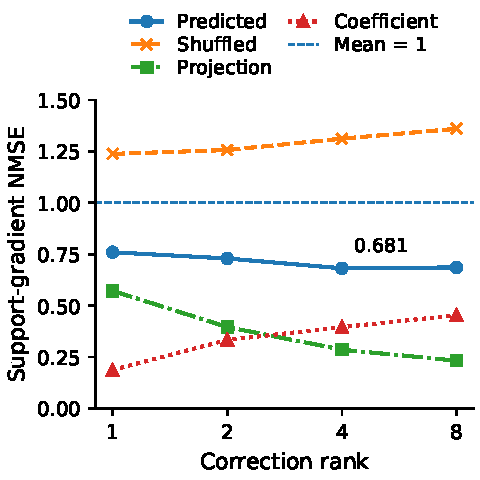
\includegraphics[width=\linewidth]{figures/latest/f1_full.pdf}\\
\textbf{\small(a) Full}
\end{minipage}\hfill
\begin{minipage}[t]{.485\linewidth}\centering
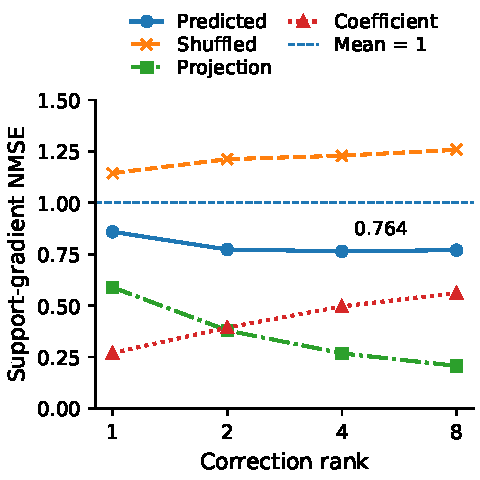
\includegraphics[width=\linewidth]{figures/latest/f1_lp1.pdf}\\
\textbf{\small(b) LP1}
\end{minipage}
\caption{\textbf{RQ3: predictable corrections, not only compressible targets.} Acoustic prediction beats the fixed-mean and shuffled-pairing references. Projection and coefficient errors describe complementary parts of total gradient-prediction error. Values are in Table~\ref{tab:f1_all}; normalization is defined in Appendix~\ref{app:rq3}.}
\label{fig:predictability}
\end{figure}

Table~\ref{tab:f1_all} shows that the comparison holds across the complete rank range. Acoustic prediction stays below the fixed-mean NMSE of one at ranks 1, 2, 4, and 8 on both input conditions; shuffled-pairing errors stay above one throughout. For Full, prediction error falls from .7595 at rank one to .6813 at rank four; LP1 falls from .8588 to .7641. The benefit therefore is not confined to a single displayed rank. The shuffled control uses the same prediction machinery but breaks the training correspondence between acoustic features and correction targets. Its larger error supports the value of that correspondence rather than attributing the improvement solely to a low-rank target representation.

The low-rank analysis explains a useful trade-off. Increasing rank from four to eight on Full reduces projection NMSE from .2858 to .2323, but increases coefficient-prediction error from .3955 to .4535, leaving total error slightly higher (.6813 to .6858). LP1 follows the same pattern. Retaining more target directions can make their coefficients harder to predict from limited support. This supports a compact predictor in the examined setting, rather than a universal optimal rank.


\paragraph{Does prediction recover the corrective direction?}
Squared error combines discrepancies in direction and magnitude. The saved held-out analysis also reports mean cosine similarity between predicted and measured gradient vectors (Table~\ref{tab:f1_all}). On Full, cosine increases from .1986 at rank one to .4092 at rank four; on LP1 it increases from .1756 to .3580. The predictor therefore recovers directional structure as well as reducing error relative to the mean. Cosines remain well below one, so this is partial recovery rather than an exact reconstruction of each recording's corrective field.

\begin{table}[t]
\caption{\textbf{RQ3: complete prediction errors and directional alignment.} All NMSE columns share the fixed-mean reference of one. Shuffled breaks training feature--gradient pairings. Cosine compares predicted and held-out correction directions; higher is better.}
\label{tab:f1_all}
\centering\small
\begin{tabular}{@{}lrrrrrr@{}}
\toprule
Input & Rank & Projection & Coefficient & Prediction & Shuffled & Cosine \\
\midrule
Full & 1 & .5719 & .1875 & .7595 & 1.2373 & .1986 \\
 & 2 & .3957 & .3334 & .7291 & 1.2563 & .2931 \\
 & 4 & .2858 & .3955 & .6813 & 1.3115 & .4092 \\
 & 8 & .2323 & .4535 & .6858 & 1.3595 & .4475 \\
\midrule
LP1 & 1 & .5887 & .2700 & .8588 & 1.1439 & .1756 \\
 & 2 & .3794 & .3932 & .7726 & 1.2118 & .2967 \\
 & 4 & .2679 & .4962 & .7641 & 1.2286 & .3580 \\
 & 8 & .2071 & .5625 & .7696 & 1.2574 & .4208 \\
\bottomrule
\end{tabular}
\end{table}

Rank eight raises cosine further, to .4475 on Full and .4208 on LP1, although total NMSE is slightly worse than at rank four. The two summaries thus favour different aspects of the update: more directions can improve average angular alignment while increasing error in the predicted coordinates or their magnitudes. This complements the development-grid result in RQ2: correction capacity should be judged against its intended endpoint, rather than selected solely from the variance captured by SVD. The local loss argument in Appendix~\ref{app:math} motivates measuring direction, while RQ1 independently tests whether a finite predicted update changes the actual answer.

RQ3 evaluates gradients, not recognition accuracy. Together, the three RQs establish separate parts of the construction: the complete pipeline improves native recognition in RQ1, relative-norm controls support input conditioning in RQ2, and held-out prediction supports the learned acoustic map in RQ3. Their distinct protocols prevent one endpoint from being substituted for another.

\section{Discussion and Scope}
\label{sec:discussion}
The results distinguish an acoustic representation that supports classification from a particular mechanism that uses it to answer. \method\ provides one such mechanism: support supervision defines internal corrections, and a compact acoustic predictor supplies them for new recordings. The improvement is measured through the original decoder, rather than through a replacement classifier. Spectral decision drift is an external-readout diagnostic; the recognition gain does not itself measure closure of that readout-transfer deficit or establish a unique cause of native errors.

The principal gain uses error-enriched support and overlapping recording-group draws. The evidence covers one model family. In a separate class-balanced fixed-setting study, 7B/LP1 improves from 14.43\% to 17.53\% accuracy but loses macro-F1; Full and both 3B conditions show no accuracy gain, and off-diagonal correction-map transfer does not exceed shuffled controls in accuracy. Direct ridge readouts are stronger for fixed-label classification in that study (Appendix~\ref{app:extensions}). These outcomes limit generalization without replacing the main operating-point result: the support policy, feature layers, and update normalization differ together, so their individual effects are not isolated. MarmAudio also lacks clip-level caller identities, and its recognition labels do not establish animal communicative meaning.

\section{Conclusion}
We study how existing acoustic information can influence a speech language model's own recognition answers. Matched-support and spectral probes motivate \method, a supervised regression from acoustic features to additive internal corrections. The main evaluation improves mean native accuracy by 20.12 points, with higher macro-F1 and gains in every recording-group draw. Conditioning controls and held-out target prediction support the design, while separate transfer and scale tests describe its operating scope.
\label{maintextend}

\clearpage
\subsection*{AI use statement}
Generative AI tools assisted manuscript drafting and revision, figure-design specifications, and development of research software and verification scripts. This revision reorganizes the supplied experimental evidence and does not add model evaluations. Quantitative results, software checks, and scientific experiments are treated separately. The authors are responsible for the final submitted text, figures, software, and claims.

\subsection*{Ethics statement}
This work reuses existing animal-sound datasets and conducts no new animal experiments. Recordings are subject to their dataset-specific licensing and redistribution terms. Recognition concerns supplied call-type, caller, and species labels; it does not establish translations, intentions, or validated communicative responses. Ecological or welfare deployment would require population- and environment-specific validation.

\subsection*{Reproducibility statement}
Appendix~\ref{app:protocols} maps datasets, sample selection, and settings to each research question. Appendices~\ref{app:diagnosis}--\ref{app:variants} give diagnostic definitions, the algorithm, complete supporting results, extensions, and variant identities. The source package contains the manuscript, figure assets, bibliography, and scalar data snapshots used for reported plots. Raw audio, model weights, and large intermediate tensors are not bundled. Author-facing source and editorial records are separate from the anonymous manuscript.

\begingroup
\small
\bibliography{references}
\bibliographystyle{iclr2027_conference}
\endgroup
\clearpage
\appendix

\section{Data and Evaluation Protocols}
\label{app:protocols}
\label{app:tasks}
This appendix separates dataset identity from experimental role. MA-CT, BD-ID, and BW-SP abbreviate existing recognition tasks, not new benchmarks. The same dataset appears in several protocols because explicit-readout diagnosis, deployed correction, and gradient prediction answer different questions. Sample counts and baseline scores are not interchangeable across those protocols.

\subsection{Datasets, classes, and labels}
\begin{table}[htbp]
\caption{\textbf{Evaluated datasets and recognition targets.} Counts describe the subsets used here, not each source collection's full size. Training/validation/test counts follow the released BEANS splits.}
\label{tab:datasets}
\centering\small
\begin{tabular}{@{}L{2.5cm}L{3.0cm}L{2.8cm}L{4.4cm}@{}}
\toprule
Dataset & Label denotes & Evaluated data & Role \\
\midrule
MarmAudio (MA-CT) \citep{lamothe2025marmaudio} & Six call types in one species & 546 expert-agreed clips & Motivation, RQ1, RQ3, and fixed-setting extensions \\
BEANS Dogs (BD-ID) \citep{hagiwara2022beans} & Ten individual dogs & 415/139/139 clips & Matched-support diagnosis and RQ2 controls \\
BEANS Watkins (BW-SP) \citep{hagiwara2022beans} & 31 marine-mammal species & 1,017/339/339 clips & Spectral readout diagnosis and full-training references \\
\bottomrule
\end{tabular}
\end{table}

The MA-CT subset contains recordings affirmed by all four annotators in the technical-validation release. Its six labels are Infant Cry, Phee, Seep, Trill, Tsik, and Twitter. The Phee, Trill, and Twitter contours in Figure~\ref{fig:motivation}a are schematic representations of spectrotemporal structure \citep{dimattina2006virtual,agamaite2015quantitative}, not measured spectrograms or statements about communicative meaning. MarmAudio does not assign a caller identity to each clip. Recording-disjoint evaluation therefore does not establish performance on unseen callers.

A support example is one recording and its task label. In MA-CT, two examples per class mean two clips of each call type: twelve clips from one species, not two animals. In BD-ID, an individual is the class, so two examples are two clips from the same named dog; the full two-shot support contains twenty clips. In BW-SP, two examples per class would mean two clips per species, or 62 clips, without requiring distinct individuals within a species. This last definition describes a support convention, not a claim that the completed study includes a 62-support Watkins AKR experiment.

Semantic labels and consistently remapped symbolic labels are evaluated separately. A--F mappings on MA-CT and A--J mappings on BD-ID associate the same acoustic classes with alternative output symbols. These controls test the demonstrated association rather than familiarity with category names. They do not change the underlying recognition labels for scoring.

\subsection{One protocol per scientific comparison}
\begin{table}[htbp]
\caption{\textbf{Protocol-to-question map.} Full-data probe fitting, small-support ICL, error-enriched correction, and class-balanced extensions have different sample budgets. Within a row, the indicated comparators share evaluation identities.}
\label{tab:protocol_map}
\centering\small
\begin{tabular}{@{}L{2.15cm}L{3.4cm}L{3.65cm}L{3.5cm}@{}}
\toprule
Purpose & Support or training data & Evaluation data & Comparators / endpoint \\
\midrule
Matched support & MA-CT: $k=1,2,4,8,16$ per class; nested support & Same 75 recording-disjoint queries & Ridge/centroid; measured ICL at $k=1,2$; accuracy \\
Spectral diagnosis & Condition-specific training features; MA-CT grouped out-of-fold; BEANS released splits & MA-CT 546 out-of-fold predictions; BD-ID 139 and BW-SP 339 test clips & Native, condition-fitted, and transferred readouts \\
RQ1 recognition & MA-CT: 20 total error-enriched clips, one per support recording & Five draws of 39, 64, 57, 68, and 82 LP1 queries & Native, fixed mean, continuous AKR; accuracy/macro-F1 \\
RQ2 controls & BD-ID: 2 clips per dog, 20 total & Same 139 validation queries at each strength & Fixed, pooled, ordered, permuted, random; accuracy \\
RQ3 prediction & MA-CT: 48 class-balanced clips from 32 recording groups & Five held-out folds within support & Predicted, mean, and shuffled targets; NMSE \\
Transfer/scale & Same 48 class-balanced MA-CT support clips; 7B/3B fitted separately & Same 97 recording-separated query clips for Full/LP1 & Native, fixed, AKR, ridge; transfer also includes shuffled fields \\
\bottomrule
\end{tabular}
\end{table}

\paragraph{RQ1 selection.}
The main recognition protocol selects twenty total support clips, one per source recording, from the available pool answered correctly at Full but incorrectly at LP1. Query recording groups are drawn first from all 93 groups, before checking failure eligibility. Ten query groups are drawn and all their events are evaluated. Support and query recordings are disjoint within each draw; the five draws may overlap with one another. This error-enriched support selection is not the class-balanced $k$-per-class protocol used for ICL or the later fixed-setting study.

\paragraph{RQ2 identity.}
The conditioning table uses the recorded continuous-field Dogs validation comparison, with three active-block relative strengths. Ordered tokenwise and token-permuted fields remain part of that comparison. A separate class-routed A--J sweep is not substituted into these rows. The historical feature-depth/rank grid also has its own query set and is reported separately in Appendix~\ref{app:rq2}.

\paragraph{RQ3 and extension identity.}
The completed fixed-setting study records seed 20260914 and eight support clips per call type. Its prediction analysis holds out support recording groups; its recognition extensions use 97 separate queries. The held-out fold sizes are 9, 9, 13, 11, and 6. A new normalizer, basis, and ridge map are fitted within each training fold. No recognition-query gradient is used in this analysis. The same support and query identities are reused across Full/LP1 and 7B/3B in the extensions, but each model has its own features and correction targets. These data had been inspected previously; the study is a fixed-setting extension, not a new untouched test.

\begin{table}[htbp]
\caption{\textbf{Recorded fitting and generation settings.} Feature indices are the stored backend indices, not names for the intervention layers. Unreported historical layer lists are not inferred from the separate development grid or later extension.}
\label{tab:settings}
\centering\small
\begin{tabular}{@{}L{3.35cm}L{9.65cm}@{}}
\toprule
Protocol & Setting \\
\midrule
RQ1 & Feature index 0; rank 4; ridge penalty 10; raw $\eta=300$; draw seeds 20250813--20250817 \\
RQ2 & Active-block relative strengths $.003$, $.01$, $.03$; same recorded support and query set across fields \\
RQ3 & 7B feature index 24; K/V layers 7, 14, 21, 24; diagnostic ranks 1, 2, 4, 8; ridge penalty 10; five recording-group folds \\
7B extension & Feature index 24; K/V layers 7, 14, 21, 24; rank 4; ridge penalty 10; $\alpha=.01$ \\
3B extension & Feature index 32; K/V layers 9, 18, 27, 31; rank 4; ridge penalty 10; $\alpha=.01$ \\
Recognition & Frozen Thinker, Talker disabled; BF16; batch size 1; greedy text generation \\
Extension hardware & One RTX 4090; 24-GB placement profile; direct Thinker with SDPA attention \\
\bottomrule
\end{tabular}
\end{table}

The extension uses a fixed numerical setting, not historical validation-selected parameters. Relative depth gives different layer indices at different scales; no 7B tensors are copied into 3B. The exported protocol specifies the following checkpoint revisions:
\begin{quote}\small\ttfamily
7B: ae9e1690543ffd5c0221dc27f79834d0294cba00\\
3B: f75b40e3da2003cdd6e1829b1f420ca70797c34e
\end{quote}
The execution record lists Torch 2.13.0+cu130 and Transformers 4.52.3. Large intermediate arrays, raw audio, and model weights are not included in the manuscript package. The source snapshot does not enumerate every historical intervention layer or every per-draw sample identity in the manuscript itself; the corresponding saved run artifacts remain the authority for those details.

\subsection{Audio processing and scoring}
Filtering is applied at each recording's source sampling rate before anti-alias resampling to 16\,kHz. Full therefore denotes the model-observable 0--8\,kHz baseband, not the original 0--48\,kHz range of a 96-kHz MarmAudio recording. LP1/2/4/6/8 denote low-pass cutoffs of 1/2/4/6/8\,kHz. LP8 is a filtered control, distinct from unfiltered Full. Per-condition peak normalization is disabled; RMS-matched controls are separate. Low-pass filtering changes the available spectrum without relabelling the vocalization or shifting its entire pitch trajectory.

Accuracy counts invalid or multiple-label outputs as incorrect. Macro-F1 complements overall accuracy with class-balanced performance \citep{sokolova2009systematic}. When paired predictions are available, a repair is a previously incorrect answer becoming correct, and a damage is a previously correct answer becoming incorrect. With $R$ repairs and $H$ damages over $N$ queries, the accuracy change is $(R-H)/N$. Repeated recording draws use descriptive means and sample SD, not confidence intervals that treat overlapping observations as independent. Single-seed extensions have no between-seed error bars, and shared transfer/scale operating points are counted once.

\clearpage
\section{Exploratory Diagnostics}
\label{app:diagnosis}
\label{sec:diagnosis}
\label{app:motivation_protocol}
These measurements support the observations in Figure~\ref{fig:motivation}; they precede the three method-evaluation questions. Matched-support ICL measures supervision use, while spectral probes measure readout transfer. Neither diagnostic is an objective optimized by AKR.

\subsection{Matched-support recognition}
For a $C$-class task, let $\Sset_k$ contain $k$ labelled recordings per class and $\Qset$ contain held-out recordings from the same label set. An explicit readout $\widehat f_{\Sset_k}$ fits support feature--label pairs. Audio ICL instead receives the corresponding audio--answer demonstrations in its context. With a fixed prompt, the gap is
\begin{equation}
\begin{aligned}
G(k)={}&\operatorname{Acc}_{\Qset}(\widehat f_{\Sset_k}\circ h_\theta)\\
&-\operatorname{Acc}_{\Qset}\bigl(f^{\rm ICL}_\theta(\cdot;\Sset_k,p)\bigr).
\end{aligned}
\label{eq:gap}
\end{equation}
Both routes keep the speech model frozen, but only the explicit readout fits classifier parameters. The comparison matches recordings and labels, not optimization or computational cost. The concrete two-shot MA-CT episode supplies two clips of each of its six call types and evaluates both routes on the same 75 recording-disjoint queries.

\begin{table}[htbp]
\caption{\textbf{Matched-support MA-CT recognition.} Accuracy (\%) on the same 75 queries. Larger support sets follow the nested order. A dash denotes no matched ICL value used here, not zero accuracy.}
\label{tab:support_scaling}
\centering\small
\begin{tabular}{@{}rrrrr@{}}
\toprule
$k$/class & Support clips & Audio ICL & Centroid & Ridge \\
\midrule
1 & 6 & 8.00 & 29.33 & 46.67 \\
2 & 12 & 17.33 & 46.67 & 58.67 \\
4 & 24 & --- & 50.67 & 73.33 \\
8 & 48 & --- & 78.67 & 84.00 \\
16 & 96 & --- & 76.00 & 82.67 \\
\bottomrule
\end{tabular}
\end{table}

The one- and two-shot gaps are 38.67 and 41.33 percentage points, with paired 95\% intervals [25.33, 52.00] and [28.00, 54.67]. The ridge curve plateaus near eight examples per class in this evaluation; it is not a fitted scaling law. BD-ID gives a separate matched-support example: one clip per dog yields 35.25\% for ridge and 7.19\% for audio ICL on 139 validation queries.

Candidate scoring uses label-string log-likelihoods rather than free decoding, following likelihood-based few-shot evaluation \citep{brown2020language}. Audio demonstrations follow the audio-ICL setting studied by \citet{kong2024audioflamingo}; this is an evaluation on Qwen, not an Audio Flamingo backbone experiment. Sequence-sum and mean-token candidate scores are distinct because label strings have different lengths. Nearest-centroid classification compares query features with support class centroids, while ridge learns a linear feature-to-class map \citep{hoerl1970ridge,hastie2009elements}.

\begin{table}[htbp]
\caption{\textbf{Zero-support candidate scoring on all 546 MA-CT clips.} Full-input accuracy and macro-F1 (\%). These rows do not use the 75-query matched-support protocol.}
\label{tab:candidates}
\centering\small
\begin{tabular}{@{}lrr@{}}
\toprule
Readout & Accuracy & Macro-F1 \\
\midrule
Free generation & 29.49 & 21.94 \\
Bare candidates, token mean & 30.95 & 20.26 \\
Bare candidates, sequence sum & 33.88 & 25.36 \\
Definitions, token mean & 22.34 & 10.46 \\
Definitions, sequence sum & 18.86 & 6.58 \\
\bottomrule
\end{tabular}
\end{table}

Prompt and label preferences can affect few-shot predictions \citep{zhao2021calibrate}. In the recorded A--F controls, six counterbalanced mappings give 17.33\% one-shot candidate accuracy, within the shuffled-association range 15.33--17.78\%. Formatting or candidate scoring alone therefore does not establish effective acoustic-to-symbol learning in that protocol. These rows remain separate from semantic-label ICL and from the new gradient-prediction study.

\subsection{Spectral readout transfer}
\label{app:spectral}
Let $F_c$ be a low-pass filter and $h_c(x)=h_\theta(F_c x,p)$. Fit $f_c$ on condition-$c$ training features and $f_F$ on Full training features, then evaluate both on identical filtered queries:
\begin{equation}
D(c)=\operatorname{Acc}_{\Qset}(f_c\circ h_c)
-\operatorname{Acc}_{\Qset}(f_F\circ h_c).
\label{eq:drift}
\end{equation}
This operational transfer deficit is the quantity called spectral decision drift. Negative values are retained when the transferred readout performs better. It is not an information-theoretic decomposition or a direct measurement of a boundary inside the native decoder.

MA-CT uses nested recording-grouped out-of-fold evaluation over its 546 expert-agreed clips; each recording is excluded from fitting the readout used to predict it. BD-ID and BW-SP use their declared fixed splits. The two-shot MA-CT example does not supply the training budget for these spectral probes.

\begin{figure}[htbp]
\centering
\begin{minipage}[t]{.327\linewidth}\centering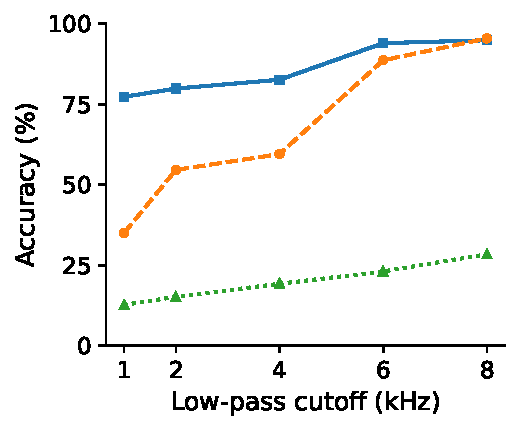
\includegraphics[width=\linewidth]{figures/fig3_marmaudio.pdf}\\\textbf{\small(a) MA-CT}\end{minipage}\hfill
\begin{minipage}[t]{.327\linewidth}\centering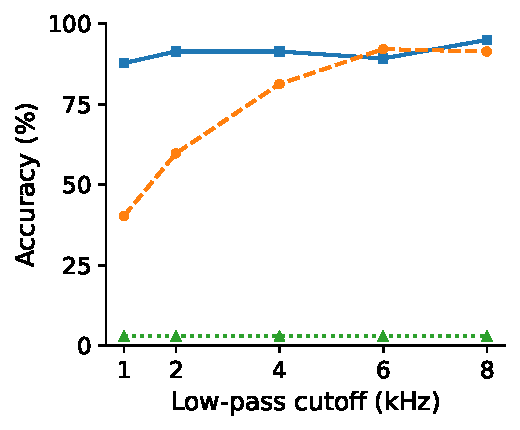
\includegraphics[width=\linewidth]{figures/fig3_dogs.pdf}\\\textbf{\small(b) BD-ID}\end{minipage}\hfill
\begin{minipage}[t]{.327\linewidth}\centering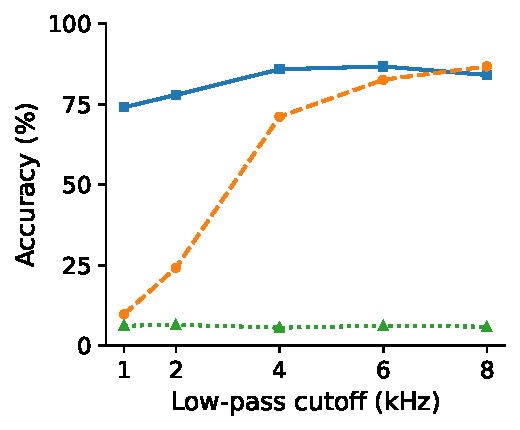
\includegraphics[width=\linewidth]{figures/fig3_watkins.pdf}\\\textbf{\small(c) BW-SP}\end{minipage}
\caption{\textbf{Retained discrimination and readout transfer.} Condition-fitted and Full-trained readouts score identical filtered queries; native generation is shown separately. The LP8 filtered control is not unfiltered Full.}
\label{fig:spectrum}
\end{figure}

\begin{table}[htbp]
\caption{\textbf{Complete spectral readout values.} Each triplet is native / condition-fitted / Full-trained transferred accuracy (\%).}
\label{tab:spectral}
\centering\small
\begin{tabular}{@{}rccc@{}}
\toprule
Cutoff & MA-CT & BD-ID & BW-SP \\
\midrule
1 kHz & 12.64 / 77.29 / 34.98 & 2.88 / 87.77 / 40.29 & 6.19 / 74.04 / 9.73 \\
2 kHz & 15.20 / 79.85 / 54.58 & 2.88 / 91.37 / 59.71 & 6.49 / 77.88 / 24.19 \\
4 kHz & 19.23 / 82.60 / 59.52 & 2.88 / 91.37 / 81.29 & 5.60 / 85.84 / 71.09 \\
6 kHz & 23.08 / 93.96 / 88.64 & 2.88 / 89.21 / 92.09 & 6.19 / 86.73 / 82.60 \\
8 kHz & 28.39 / 94.87 / 95.42 & 2.88 / 94.96 / 91.37 & 5.90 / 84.07 / 86.73 \\
\bottomrule
\end{tabular}
\end{table}

\paragraph{Bidirectional and shared-setting controls.}
\label{app:extended_spectral}
Transfer also fails when a low-pass-trained readout receives Full features. Table~\ref{tab:bidirectional} reports each source readout's matched accuracy and transfer accuracy. Shared-setting controls fix feature layer and ridge regularization across sources while still fitting readout coefficients on each source. Their deficits show that different layer/regularization choices are not sufficient to explain the pattern.

\begin{table}[htbp]
\caption{\textbf{Bidirectional readout transfer.} Accuracy (\%) on the declared BD-ID/BW-SP test splits. The source-matched reference and target-matched matrix reference below are different comparisons.}
\label{tab:bidirectional}
\centering\small
\begin{tabular}{@{}llrrr@{}}
\toprule
Task & Source $\to$ target & Source-matched & Transferred & Shared-setting transfer \\
\midrule
BD-ID & Full $\to$ LP1 & 92.81 & 40.29 & 40.29 \\
BD-ID & LP1 $\to$ Full & 87.77 & 38.85 & 30.22 \\
BW-SP & Full $\to$ LP1 & 88.20 & 9.73 & 9.73 \\
BW-SP & LP1 $\to$ Full & 74.04 & 20.35 & 23.01 \\
\bottomrule
\end{tabular}
\end{table}

For the complete matrices, write $M_{s,t}$ for accuracy of a readout fitted at source bandwidth $s$ and evaluated at target $t$. The target-referenced deficit is
\begin{equation}
D_{s,t}=M_{t,t}-M_{s,t}.
\label{eq:matrixdeficit}
\end{equation}
Each column uses the same target recordings. Its diagonal is zero by definition. For BD-ID, Full$\to$LP1 gives $87.77-40.29=47.48$ points; for BW-SP it gives $74.04-9.73=64.31$ points. These are readout-transfer measurements, not AKR repair scores.

\begin{figure}[htbp]
\centering
\begin{minipage}[t]{.49\linewidth}\centering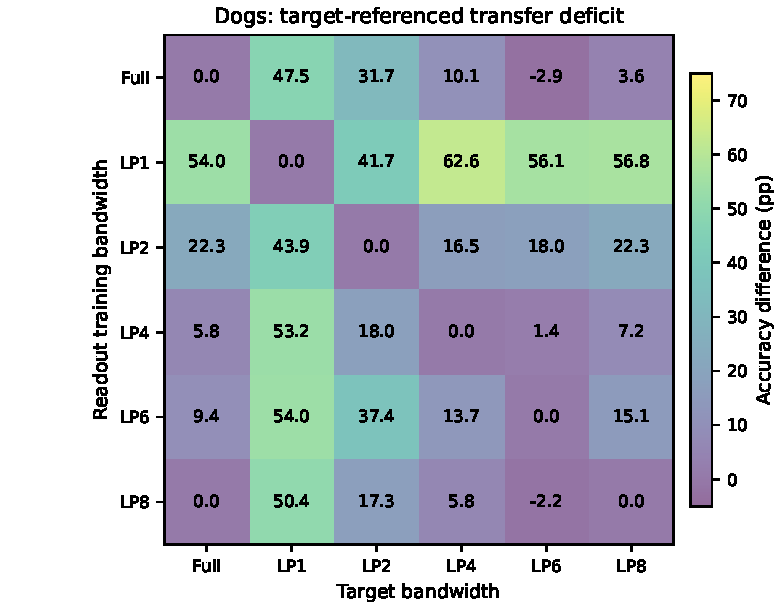
\includegraphics[width=\linewidth]{figures/analysis/01_dogs_transfer_deficit.pdf}\\\textbf{\small(a) BD-ID}\end{minipage}\hfill
\begin{minipage}[t]{.49\linewidth}\centering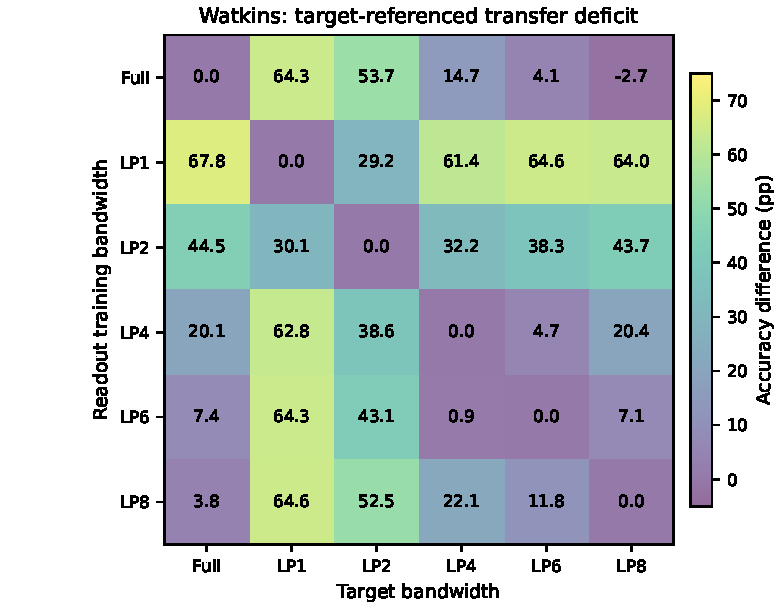
\includegraphics[width=\linewidth]{figures/analysis/01_watkins_transfer_deficit.pdf}\\\textbf{\small(b) BW-SP}\end{minipage}
\caption{\textbf{Target-referenced spectral deficits.} Each cell is Eq.~\ref{eq:matrixdeficit} in percentage points. Positive values mean that transferring a source readout underperforms fitting at the target condition.}
\label{fig:transfermatrices}
\end{figure}

\paragraph{Additional signal checks.}
On a separate balanced 300-event MA-CT subset, cyclic audio substitution scores 16.67\% against the original labels and 30.33\% against the substituted recording's labels; the latter equals the canonical unmodified-audio accuracy. Silence scores 15.00\% and favours a small label subset. RMS matching raises LP1 native accuracy from 12.33\% to 18.33\% on that subset. Attenuation contributes, but these controls do not make all spectral effects an amplitude effect. Across five cutoffs, MA-CT's transfer deficit and correction-target rotation have Spearman $\rho=1.00$ and Pearson $r=.969$. Both vary with bandwidth, so this is an association rather than causal mediation. The more extensive score-transform plots in the source materials are redundant views of these measurements, not additional experiments.

\clearpage
\section{Method and Implementation Details}
\label{app:math}
\begin{algorithm}[htbp]
\caption{\method: support fitting and label-free query inference}
\label{alg:akr}
\begin{algorithmic}[1]
\Require Frozen model $\theta$, labelled support $\Sset$, rank $r$, ridge penalty $\lambda$, raw step $\eta$
\For{each $(x_i,y_i)\in\Sset$}
\State Extract $h_i$ from $(x_i,p)$ without the answer label.
\State Compute answer loss and pooled negative K/V target $g_i$ using Eqs.~\ref{eq:answerloss}--\ref{eq:gradient}.
\EndFor
\State Fit support feature normalizers and compute $\bar g,B,a_i$ using Eq.~\ref{eq:svd}.
\State Fit $W,b$ with Eq.~\ref{eq:regression}; retain all fitted objects unchanged for evaluation.
\For{each unlabelled query $x_q$}
\State Extract and standardize $h_q$ in a first forward pass.
\State Predict $\widehat g_q$ with Eq.~\ref{eq:prediction} and unflatten it into K/V blocks.
\State Run the same recording/prompt again with audio-position increments from Eq.~\ref{eq:update}.
\State Generate the original decoder's answer; use the label only for subsequent scoring.
\EndFor
\end{algorithmic}
\end{algorithm}

\subsection{Targets, coordinates, and parameter shapes}
The answer-token cross-entropy defines an error signal for the frozen speech model. Its negative state gradient defines a real-valued correction target. Fitting $W,b$ then minimizes squared coordinate error, not class cross-entropy or a policy-distillation loss. For $n$ support recordings, feature width $d$, gradient width $P$, and retained rank $r$, the shapes are $G\in\R^{n\times P}$, $B\in\R^{P\times r}$, $W\in\R^{r\times d}$, and $b\in\R^r$. The standardizer uses $z_{ij}=(h_{ij}-\mu_j)/\sigma_j$ with support-only statistics, replacing very small scales by one. Ridge penalizes $W$, not its intercept. One support recording has no centred target variation, so its conditional correction reduces to the fixed mean.

The selected hooks operate on projection outputs before head reshaping. Key increments precede rotary position encoding; values do not undergo that key rotation. Audio pooling excludes text and answer positions from the target and from direct additive injection. Subsequent attention can still propagate the effect to the answer. A shared basis compresses correction targets; the original states remain present in the additive update.

\subsection{Projection and coefficient-prediction error}
\label{app:predictability}
For analysis, let $a_q=B^\top(g_q-\bar g)$ denote coordinates of a labelled held-out gradient. With $B^\top B=I$, orthogonality gives
\begin{equation}
\begin{aligned}
\norm{g_q-\widehat g_q}_2^2
={}&\norm{(I-BB^\top)(g_q-\bar g)}_2^2\\
&+\norm{a_q-(Wz_q+b)}_2^2.
\end{aligned}
\label{eq:decomposition}
\end{equation}
The first term measures target variation omitted by the basis; the second measures prediction error in retained coordinates. A small projection residual does not establish predictability. RQ3 evaluates both terms on held-out support groups, where labels may be used for analysis; labelled recognition-query gradients are not required at deployment. The decomposition is exact for the defined Euclidean coordinates and does not imply an accuracy guarantee.

\subsection{Local loss interpretation}
Let $T_i$ broadcast a pooled block vector across a recording's audio positions. Eq.~\ref{eq:gradient} gives $T_i^\top\nabla_Z\mathcal L_i=-|\Aset_i|g_i$. For a small raw step,
\begin{equation}
\mathcal L_i(Z+\eta T_i\widehat g_i)-\mathcal L_i(Z)
=-\eta|\Aset_i|\langle g_i,\widehat g_i\rangle+O(\eta^2).
\label{eq:local}
\end{equation}
Positive alignment favours locally lower loss. Finite updates, sequential attention effects, numerical precision, and discrete decoding can change the observed answer. This explains the support target; it does not justify estimating a labelled recognition-query gradient during inference or guarantee that every predicted update is helpful.

\subsection{Relative-norm controls and variant identities}
For an active layer/projection/scope block, relative scaling is
\begin{equation}
\Delta Z_{\rm rel}=
\begin{cases}
\displaystyle\alpha\frac{\norm{Z_{\rm active}}_F}{\norm{\Delta Z}_F}\Delta Z,
&\norm{\Delta Z}_F>0,\\[3pt]
0,&\text{otherwise}.
\end{cases}
\label{eq:relative}
\end{equation}
The ratio is recorded per active block. Equal per-block ratios do not imply equal total energy when the number of layers or scope changes. These controls do not retroactively norm-match RQ1's raw-step comparison. Zero direction or zero strength is a strict no-op.

Continuous AKR predicts real-valued coefficients without first choosing a class. A class-routed dictionary instead predicts a class and retrieves its support-gradient centroid. Pooled targets share a block vector across audio positions; ordered tokenwise targets retain position-resolved fields. These choices define different variants whose results are not interchanged. Appendix~\ref{app:variants} contains the separate class-routed and Oracle results.

\clearpage
\section{Full Results for RQ1--RQ3}
\label{app:fullresults}
\subsection{RQ1: recording-group results and class-resolved changes}
\label{app:rq1}
\label{app:repair_draws}
The five rows of Table~\ref{tab:draws} correspond, in order, to seeds 20250813--20250817 and query counts 39, 64, 57, 68, and 82.


The mean paired accuracy differences are $20.12\pm8.02$ points against native generation and $19.46\pm5.15$ against fixed mean (sample SD across draws). Each difference is positive in every draw. This comparison reports the recorded raw-step operating point, not a sweep over newly selected parameters.

\paragraph{Complete first-draw class analysis.}
\label{app:case}
\label{app:decisionchanges}
The first numerically indexed draw, seed 20250813, includes all 39 queries. Its paired class analysis compares continuous AKR with fixed mean, not with native generation. Table~\ref{tab:classes} in the main text shows every class, including unresolved categories. The paired outcome partition is zero both-correct, twelve fixed-wrong/AKR-correct, two fixed-correct/AKR-wrong, and twenty-five both-wrong. These four counts sum to 39.


Phee and Twitter account for ten of the twelve AKR-correct answers. Infant Cry and Trill remain unresolved. Both methods emit four labels with zero invalid outputs. The prediction counts for Infant Cry/Phee/Seep/Trill/Tsik/Twitter are 0/11/1/0/24/3 for fixed mean and 0/10/5/0/13/11 for AKR. Less concentrated output accompanies higher macro-F1 (2.38\% to 23.79\%), but is not itself evidence that every class has been repaired.

\subsection{RQ2: complete controls and feature/rank context}
\label{app:rq2}
Table~\ref{tab:ablation} includes the full recorded continuous-field comparison at all three relative strengths. The same twenty support clips and 139 validation queries are used within that comparison. At $\alpha=.03$, the pooled-versus-fixed paired accuracy interval is [2.88, 13.67] points. Ordered tokenwise correction exceeds its permutation at $.01$ and $.03$, but fails its recorded stability criterion and is not uniformly superior to pooling. Invalid-rate values from the separate class-routed experiment are not assigned to these continuous-field rows.

Table~\ref{tab:rankdepth} uses twenty support clips and 64 development queries while varying feature index and requested rank. Selection prioritizes macro-F1, then accuracy, then smaller rank and earlier layer. These measurements do not initiate a new selection for RQ1, the relative-norm control, or RQ3.


The recorded selection is feature 28/rank 8.

\subsection{RQ3: held-out prediction, normalization, and decomposition}
\label{app:rq3}
\label{app:completed_f1}
Let $\mathcal H_f$ contain the held-out support clips in fold $f$, $\bar g_{-f}$ be the training-gradient mean, and $\widehat g_{-f}(h_i)$ the predictor fitted on that training portion. The normalization is
\begin{equation}
\operatorname{NMSE}=
\frac{\sum_f\sum_{i\in\mathcal H_f}\norm{g_i-\widehat g_{-f}(h_i)}_2^2}
{\sum_f\sum_{i\in\mathcal H_f}\norm{g_i-\bar g_{-f}}_2^2}.
\label{eq:nmse}
\end{equation}
Numerators and denominators are summed across folds before division; the result is not an unweighted average of separately normalized fold errors. The same denominator is used for projection and coefficient errors. Their sum equals total prediction error up to rounding. No group crosses a training/held-out boundary, and normalization, SVD, and ridge are all refitted on each fold's training clips.


Table~\ref{tab:f1_all} reports all results. Cosine averages the 48 nonzero held-out support gradients; projection and coefficient terms follow Eq.~\ref{eq:decomposition}.

A true-class-centroid control reaches NMSE .3572 on Full and .2950 on LP1, with no missing-class fallback. It uses each held-out support label to select the centroid and is therefore a label-using diagnostic, not a deployable query method. It describes target label structure without implying that the regressor receives query labels. Prediction NMSE and final recognition need not agree: one measures squared error in update coordinates, the other measures a discrete decoder decision after a finite perturbation. Appendix~\ref{app:extensions} evaluates that downstream behaviour separately.

\clearpage
\section{Transfer, Model Scale, and Direct Readouts}
\label{app:extensions}
\label{app:closing_protocol}
The class-balanced fixed-setting study tests how the correction map behaves beyond the main error-enriched operating point. Full and LP1 use the same 48 support clips and 97 query clips. Rank four, ridge penalty ten, and $\alpha=.01$ are fixed; settings and model-specific indices are listed in Appendix~\ref{app:protocols}. The numerical settings do not copy tensors between model sizes. The data had been inspected previously, and the single-seed comparisons do not establish generalization across model families.

\subsection{Correction-map transfer}
\label{app:completed_f2}
Fit one continuous predictor on Full support and another on LP1 support, then apply each unchanged to Full and LP1 queries. Normalization, mean, basis, and coefficients remain fixed within a source-trained map. This tests the correction map, unlike Appendix~\ref{app:spectral}'s transfer of external classifiers.

\begin{table}[htbp]
\caption{\textbf{Complete 7B correction-map transfer.} Accuracy (\%) on the same 97 queries. Column labels are support condition $\to$ query condition. The diagonal cells are shared with the 7B scale comparison, not independent repetitions.}
\label{tab:latest_transfer}
\centering\small
\begin{tabular}{@{}lrrrr@{}}
\toprule
Method & Full$\to$Full & Full$\to$LP1 & LP1$\to$Full & LP1$\to$LP1 \\
\midrule
Native & 26.80 & 14.43 & 26.80 & 14.43 \\
Fixed mean & 25.77 & 12.37 & 24.74 & 12.37 \\
Shuffled field & 26.80 & 15.46 & 24.74 & 14.43 \\
Continuous AKR & 26.80 & 15.46 & 24.74 & 17.53 \\
Frozen ridge & 81.44 & 17.53 & 38.14 & 60.82 \\
\bottomrule
\end{tabular}
\end{table}

\begin{table}[htbp]
\caption{\textbf{Transfer metrics and paired decision changes.} Accuracy/macro-F1 are percentages; $R/H$ count repaired/damaged answers against native on the same query condition. All invalid rates are zero. Native Full is 26.80/16.53; native LP1 is 14.43/8.38.}
\label{tab:f2_complete}
\centering\small
\begin{tabular}{@{}llrrrr@{}}
\toprule
Support $\to$ query & Method & Accuracy & Macro-F1 & $R$ & $H$ \\
\midrule
Full$\to$Full & Fixed mean & 25.77 & 16.06 & 0 & 1 \\
 & Shuffled field & 26.80 & 16.26 & 1 & 1 \\
 & Continuous AKR & 26.80 & 15.86 & 2 & 2 \\
 & Frozen ridge & 81.44 & 78.21 & 56 & 3 \\
\midrule
Full$\to$LP1 & Fixed mean & 12.37 & 4.17 & 0 & 2 \\
 & Shuffled field & 15.46 & 8.36 & 1 & 0 \\
 & Continuous AKR & 15.46 & 6.89 & 2 & 1 \\
 & Frozen ridge & 17.53 & 12.28 & 12 & 9 \\
\midrule
LP1$\to$Full & Fixed mean & 24.74 & 14.82 & 0 & 2 \\
 & Shuffled field & 24.74 & 14.38 & 1 & 3 \\
 & Continuous AKR & 24.74 & 13.93 & 2 & 4 \\
 & Frozen ridge & 38.14 & 33.80 & 25 & 14 \\
\midrule
LP1$\to$LP1 & Fixed mean & 12.37 & 6.07 & 0 & 2 \\
 & Shuffled field & 14.43 & 4.86 & 2 & 2 \\
 & Continuous AKR & 17.53 & 7.47 & 4 & 1 \\
 & Frozen ridge & 60.82 & 57.12 & 48 & 3 \\
\bottomrule
\end{tabular}
\end{table}

On LP1 queries, the matched AKR map yields 17 correct answers, the Full-trained map 15, and native generation 14. On Full queries, the LP1-trained map gives 24 against 26 native. Both off-diagonal AKR accuracies equal their shuffled-field counterparts; equal accuracy does not mean identical predictions, as the paired counts show. Matched LP1 has a local advantage over shuffled fields, but this does not establish cross-spectral invariance.

\subsection{Within-family scale comparison}
\label{app:completed_f3}
\begin{table}[htbp]
\caption{\textbf{Backbone-grouped comparison under identical supervision.} Accuracy and macro-F1 (\%) on MA-CT, with the same support/query identities and fixed numerical settings. Each model fits its own map. Ridge is a direct classifier, not a KV correction.}
\label{tab:backbone_results}
\centering\small
\begin{tabular}{@{}L{2.4cm}L{2.7cm}rrrr@{}}
\toprule
& & \multicolumn{2}{c}{MA-CT / Full} & \multicolumn{2}{c}{MA-CT / LP1} \\
\cmidrule(lr){3-4}\cmidrule(lr){5-6}
Backbone & Method & Acc. & F1 & Acc. & F1 \\
\midrule
\multirow{4}{2.4cm}{Qwen2.5-Omni\\7B} & Native & 26.80 & 16.53 & 14.43 & 8.38 \\
 & Frozen ridge & \textbf{81.44} & \textbf{78.21} & \textbf{60.82} & \textbf{57.12} \\
 & Fixed-mean KV & 25.77 & 16.06 & 12.37 & 6.07 \\
 & Continuous AKR & 26.80 & 15.86 & 17.53 & 7.47 \\
\midrule
\multirow{4}{2.4cm}{Qwen2.5-Omni\\3B} & Native & 27.84 & 18.60 & 16.49 & 6.06 \\
 & Frozen ridge & \textbf{84.54} & \textbf{82.37} & \textbf{69.07} & \textbf{65.36} \\
 & Fixed-mean KV & 28.87 & 19.36 & 15.46 & 5.32 \\
 & Continuous AKR & 27.84 & 18.68 & 16.49 & 6.35 \\
\bottomrule
\end{tabular}
\end{table}

\begin{table}[htbp]
\caption{\textbf{Native-to-AKR changes in the scale study.} Each row's outcome counts sum to 97; all invalid rates are zero. Deltas are percentage points.}
\label{tab:f3_transitions}
\centering\small
\begin{tabular}{@{}llrrrrrr@{}}
\toprule
Model & Input & Both right & Repair & Damage & Both wrong & $\Delta$Acc. & $\Delta$F1 \\
\midrule
7B & Full & 24 & 2 & 2 & 69 & +0.00 & -0.66 \\
7B & LP1 & 13 & 4 & 1 & 79 & +3.09 & -0.91 \\
3B & Full & 27 & 0 & 0 & 70 & +0.00 & +0.08 \\
3B & LP1 & 16 & 0 & 0 & 81 & +0.00 & +0.29 \\
\bottomrule
\end{tabular}
\end{table}

Only 7B/LP1 increases accuracy, by three net correct answers, while macro-F1 decreases. Both 3B conditions preserve the number of correct predictions; their small macro-F1 changes reflect a changed error distribution. Frozen ridge is substantially stronger in this fixed-label task. These results do not demonstrate uniform state-repair gains or cross-family generalization. They also do not repeat RQ1's support selection, feature layer, or raw-step normalization. Their smaller effects cannot be attributed to any one of those changes from the available comparison.

\clearpage
\section{Additional Baselines and Variants}
\label{app:variants}
These references clarify the available alternatives and intervention boundaries without being substituted for the continuous-AKR RQs. Full-training baselines have a different supervision budget; class-routed and Oracle methods have different prediction or label-access rules.

\subsection{Full-training recognition references}
AVES-bio provides frozen animal-vocalization features \citep{hagiwara2022aves}. Our classifiers fit its features on the declared training sets. The LoRA reference updates rank-eight adapters on query/value projections for one epoch \citep{hu2022lora}; it is a budget-specific adaptation, not an exhaustive LoRA search. Qwen, AVES, and the MarmAudio specialist also differ in accessible input spectrum and task supervision.

\begin{table}[htbp]
\caption{\textbf{Full-input references.} Accuracy (\%); supervised probe and LoRA rows are not matched-support comparisons against native generation. The MarmAudio specialist uses the original high-rate spectrum. A dash denotes an unreported cell.}
\label{tab:references}
\centering\small
\begin{tabular}{@{}L{7.6cm}rrr@{}}
\toprule
Reference & MA-CT & BD-ID & BW-SP \\
\midrule
Qwen2.5-Omni-3B, native & 20.33 & --- & --- \\
Qwen2.5-Omni-7B, native & 29.49 & 2.88 & 6.19 \\
Qwen-7B frozen probe & 95.42 & 92.81 & 88.20 \\
AVES-bio frozen probe \citep{hagiwara2022aves} & 93.41 & 83.45 & 85.84 \\
Qwen-7B full-train LoRA, one epoch \citep{hu2022lora} & --- & 25.18 & 31.56 \\
MarmAudio specialist, original spectrum \citep{lamothe2025marmaudio} & 88.64 & --- & --- \\
\bottomrule
\end{tabular}
\end{table}

Native model size also interacts with bandwidth in the historical paired sweep: 3B/7B score 17.22\%/12.64\% at LP1 but 20.33\%/29.49\% at Full. These native references are distinct from the AKR-adapted scale study and do not imply that one model size is uniformly preferable.

\subsection{Class-routed prompt transfer and stability}
\label{app:prompt}
A class-routed dictionary selects a class-specific gradient centroid using a classifier prediction. Its Dogs A--J prompt experiment reuses the same support gradients and router and changes only query wording or candidate order. Both prompt results below belong to that variant, not to the continuous regressor.

\begin{table}[htbp]
\caption{\textbf{Class-routed pooled prompt transfer.} Complete results on 139 validation queries with $\alpha=.03$. Accuracy/macro-F1 (\%); $R/H$ are changes relative to native.}
\label{tab:prompt}
\centering\small
\begin{tabular}{@{}lccrr@{}}
\toprule
Query prompt & Native Acc./F1 & Class-routed Acc./F1 & $R$ & $H$ \\
\midrule
Paraphrase & 12.95 / 7.58 & 30.94 / 24.97 & 33 & 8 \\
Reversed candidates & 10.79 / 2.01 & 18.71 / 13.45 & 22 & 11 \\
\bottomrule
\end{tabular}
\end{table}

The net gains are 17.99 and 7.91 points, with paired intervals [9.35, 26.62] and [0.00, 15.83]. Reversal gives fewer repairs and more damaged answers than paraphrase. Neither result establishes prompt invariance for continuous AKR.

\begin{table}[htbp]
\caption{\textbf{Separate class-routed A--J strength sweep.} Accuracy and available invalid-rate endpoints (\%). A dash is an unavailable endpoint, not zero.}
\label{tab:variant_stability}
\centering\small
\begin{tabular}{@{}lrrr@{}}
\toprule
Measure & $\alpha=.003$ & $\alpha=.01$ & $\alpha=.03$ \\
\midrule
Pooled accuracy & 14.39 & 18.71 & 20.14 \\
Ordered tokenwise accuracy & 15.11 & 6.47 & 0.00 \\
Token-permuted accuracy & 7.91 & 4.32 & 0.72 \\
Ordered invalid rate & 24.46 & --- & 99.28 \\
\bottomrule
\end{tabular}
\end{table}

The ordered variant becomes less accurate as strength rises and reaches 99.28\% invalid responses at $.03$. This result is retained together with the favourable prompt-transfer outcomes of the same broader variant family. It is not used to assign failure rates to the continuous pooled method.

\subsection{Label-using Oracle capacity controls}
\label{app:oracle}
\begin{table}[htbp]
\caption{\textbf{Selected twelve-event Oracle scope diagnostic.} Correct or wrong target labels are supplied to construct the update. Audio-only recovery is reported over registered strengths, not at a deployable label-free operating point.}
\label{tab:oracle}
\centering\small
\begin{tabular}{@{}L{8.8cm}L{4.0cm}@{}}
\toprule
Intervention & Recorded outcome \\
\midrule
Full-prefill, correct-label gradient & 12/12 correct \\
Full-prefill, wrong-label gradient & 11/12 driven to supplied target \\
Full-prefill, matched random & 0/12 recovered \\
Full-prefill, audio-token permutation & 12/12 correct \\
Audio-only, correct-label gradient & 5/12 recovered in sweep \\
Audio-only, token-permuted & 1/12 recovered in sweep \\
Audio-only, matched random & 0/12 recovered \\
\bottomrule
\end{tabular}
\end{table}

Full-prefill interventions can affect prompt and decision positions as well as audio positions; their success does not isolate an acoustic-token mechanism. The separate 111-event Full-correct/LP1-wrong Oracle reaches full recovery at one reported raw step, but uses query labels and is not a deployable result. The main method instead predicts audio-position increments from support-fitted acoustic regression and is evaluated without query-label gradients.

\end{document}
